The Physical Environment Virtual Subsystem is the interface with the physical environment, which is controlled by sensors and actuators. It has input values from user such as the reference velocity, steering angle and also values from odometric sensors. This Subsystem consists of a controller and a simulator. \\
	The controller runs with a period equal to the sampling period, t=T, and it will receive the left and right wheel velocities, steering angle and also if any possible collision was detected. It generates new command variables for the left and right wheels.\\
	The simulator occurs with a period shorter than the sampling period and out of phase with the controller, t = T/4 + $\phi$, for the reason that is possible a more accurate reading and there are no collisions between simulator and controller processes. It receives the new values of the command variables and generates new values for the wheels velocities, the steering angle and also if any possible collision will occur.

%Physical Environment Virtual Subsystem
\begin{figure}[!htbp]
\centering
       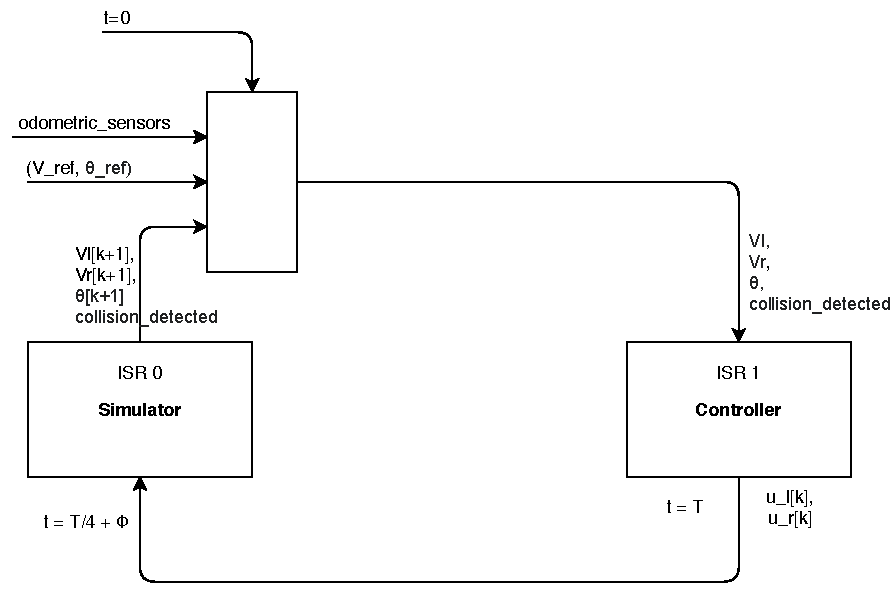
\includegraphics[width=0.8\textwidth]{img/sim&control.pdf} 
\caption{Physical Environment Virtual Subsystem}%
\label{fig:simcontroller}
\end{figure}
%
